\documentclass[10pt]{beamer}
\usepackage[slovene]{babel}
\usepackage[utf8]{inputenc}
\usepackage[T1]{fontenc}
\usepackage{lmodern}
\usepackage{mathptmx}
\usepackage{helvet}
\usepackage{courier}
\usepackage{hyperref}
\usepackage{tikz}

\usetheme{CambridgeUS}

\begin{document}

\title[Kockarjev propad ]{Kockarjev propad}
\subtitle{Gambler's ruin}
\author{Eva Deželak in Ines Šilc}
\institute [FMF]{ Fakulteta za matematiko in fiziko}

\begin{frame}
	\titlepage
\end {frame}
\section[Navodilo]{Navodilo}
\begin{frame}
\frametitle{Navodilo}
Igralec $M$ ima $m$ enot denarja, igralec $N$ pa $n$ enot premoženja, $\{m,n\}\subset \mathbb{N}$. Zapored igrata igro na srečo v kateri ni neodločenih izidov; v vsaki igri dobi zmagovalec eno denarno enoto od poraženca; igralec $M$ zmaga vsakič z verjetnostjo $p\in (0,1)$, neodvisno od preteklosti. Igranje se konča, ko eden od igralcev bankrotira. Naj bo $T$ število iger, ki so potrebne, da eden od igralcev bankrotira. 
\begin{enumerate}[(i)]
\item Določi verjetnost, da bankrotira igralec $M$. Zakaj je  $T<\infty$ s.g.?
\item Predpostavi, da je $E[T]<\infty$ (za vsako izbiro $m$ in $n$). Določi $E[T]$. *Ali znaš utemeljiti, da je $E[T]<\infty$?
\end{enumerate}

\end{frame}


\section[Posebni primeri]{Posebni primeri}
\begin{frame}
\frametitle{Končnost igre}
Vsota verjetnostii, da bankrotira igralec $M$, in da bankrotira igralec $N$:\\
\begin{equation*}
\begin{split}
&~\frac{(1-p)^{m+n}-p^m (1-p)^n}{(1-p)^{m+n}-p^{m+n}}+\frac{p^{m+n}-p^m
   (1-p)^n}{p^{m+n}-(1-p)^{m+n}} =\\
= &~\frac{(1-p)^{m+n}-p^m (1-p)^n}{(1-p)^{m+n}-p^{m+n}}-\frac{p^{m+n}-p^m
   (1-p)^n}{(1-p)^{m+n}-p^{m+n}} =\\
= &~\frac{(1-p)^{m+n}-p^m (1-p)^n-p^{m+n}+p^m
   (1-p)^n}{(1-p)^{m+n}-p^{m+n}} =\\
= &~\frac{(1-p)^{m+n}-p^{m+n}}{(1-p)^{m+n}-p^{m+n}} \\
= &~1
\end{split} 
\end{equation*}

\end{frame}

\section[Poseben primer za $p = \frac{1}{2}$]{Poseben primer za $p = \frac{1}{2}$}
\begin{frame}
\frametitle{Poseben primer za $p = \frac{1}{2}$}
Dobimo $$r = \frac{1 - \frac{1}{2}}{\frac{1}{2}} = 1.$$
V tem primeru so $u_0, u_1, \dotso, u_n$ med seboj enaki, torej:
$$u_k = r^k \cdot u_0 = u_0.$$
Posledično še lažje izrazimo $u_0$, na način:
$1 = c\cdot u_0$, torej $u_0 = \frac{1}{c}.$
V tem primeru je naša iskana verjetnost za igralca $M$ enaka:
\begin{equation*}
\begin{split}
p_m &= u_m + u_{m+1} + \cdots u_{m+n-1} = \\
		&= u_m \cdot n = \frac{n}{c} = \frac{n}{m + n}.
\end{split} 
\end{equation*}
\end{frame}

\section[Matematično upanje za $p = \frac{1}{2}$]{Matematično upanje za $p = \frac{1}{2}$}
\begin{frame}
\frametitle{Matematično upanje za $p = \frac{1}{2}$}
$$E[T|M=x] = \frac{1}{2}\cdot E[T|M=x+1] + \frac{1}{2}\cdot E[T|M=x-1] + 1,$$
\begin{equation}
\label{druga rekurzivna}
\frac{1}{2}f(x+2)-f(x+1)+\frac{1}{2}f(x)=-1
\end{equation}\\
Homogeni del:\\
$$\frac{1}{2}f(x+2)-f(x+1)+\frac{1}{2}f(x)=0$$\\
Karakteristični polinom:
\begin{equation}
\label{druga homogena}
\frac{1}{2}\lambda^2-\lambda+\frac{1}{2}=0
\end{equation} \\
Rešitev je dvojna ničla $\lambda_{1, 2}= 1$. Rešitev enačbe (\ref{druga rekurzivna}) je oblike:\\ $$(Ax+B)\cdot 1^x=Ax+B$$
\end{frame}

\begin{frame}
Nastavek za iskanje partikularne rešitve: $f(x)=C\cdot x^2\cdot 1^x= Cx^2$
 Vstavimo v enačbo (\ref{druga rekurzivna}) in dobimo:
\begin{equation*}
\begin{split}
 & ~~C(x+2)^2-2C(x+1)^2+Cx^2=-2\\
\Leftarrow & ~~C(x^2+4x+4)-2C(x^2+2x+1)+Cx^2=-2\\
\Leftarrow &  ~~C = -1 \\
\end{split}
\end{equation*}

Partikularna rešitev je $f(x)=-x^2$, splošna rešitev enačbe (\ref{druga rekurzivna}) pa je: $$f(x)=Ax+B-x^2$$

Vstavimo robne pogoje:
\begin{enumerate}
\item $f(0)=0\Rightarrow B = 0$
\item $f(m+n)=0 \Rightarrow A = m+n$
\end{enumerate}
Rešitev: $$E[T|M=x]= (m+n)x-x^2$$
Če začnemo z $m$ enotami denarja:$$E[T|M=m]=(m+n)m-m^2= n\cdot m$$
\end{frame}


\section[Posebni primeri]{Posebni primeri}
\begin{frame}
\frametitle{Posebni primeri}
\begin{enumerate}
\item V primeru, da velja $m = n$ : $$p_m = \frac{(1-p)^m}{p^m+(1-p)^m}.$$
V primeru, da je $p = \frac{1}{2}$, dobimo: 
$p_m = \frac{m}{m + m} = \frac{1}{m}.$
\item V primeru, da premoženje obeh igralcev pomnožimo s konstanto, dobimo:

$$p_m = \frac{(1-p)^{\text{cm}+\text{cn}}-(1-p)^{\text{cm}} p^{\text{cn}}}{(1-p)^{\text{cm}+\text{cn}}-p^{\text{cm}+\text{cn}}}.$$
V primeru $p = \frac{1}{2}$ torej dobimo: 
$p_m = \frac{cn}{cm + cn} = \frac{cn}{c(m + n)} = \frac{n}{m + n},$ torej ugotovimo, da se iskana verjetnost ne spremeni. 

\item $$m \to \infty  \Rightarrow p_m \to 0$$
$$n \to \infty  \Rightarrow p_m \to 1$$

\item $$p_m = \lim_{p \to 1/2}  \frac{(1-p)^{n+m} - (1-p)^m \cdot p^n}{(1-p)^{m+n} - p^{m+n}}  =\frac{n}{m + n}.$$
\end{enumerate}
\end{frame}

\section{Dokaz $E[T]<\infty$}
\begin{frame}
\frametitle{Dokaz $E[T]$<$\infty$}
Definirajmo:
\[
X_n := \left\{
\begin{array}{rl}
1; & \textrm{če zmaga igralec M}\\
0; & \textrm{če zmaga igralec N}
\end{array}
\right.
\]

Tako lahko navzgor ocenimo $T$:
$$T \leq inf\{ l \in \mathbb{N}: \textrm{v zaporedju } X_1, \dots, X_l \textrm{ smo videli } m+n \textrm{ zaporednih enic} \leq$$ 
$$
\begin{array} {lll} 
\leq (m+n)\cdot inf\{ l \in \mathbb{N}:& X_1, \dots, X_{m+n}; & \textrm{vsebuje same enice, ali} \\ 
&X_{m+n+1}, \dots, X_{2(m+n)};& \textrm{vsebuje same enice, ali}\\
&\dots \\
&X_{(l-1)(m+n)+1}, \dots, X_{l(m+n)}; & \textrm{vsebuje same enice}\}=
\end{array}$$
$\quad \quad= (m+n)\cdot G_l =: \widetilde{T}$\\

\end{frame}

\begin{frame}
Časovno os razdelimo na intervale dolžine $m+n$, znotraj katerih čakamo, da zaporedje $\{X_l\}_{l \in \mathbb{N}}$ vsebuje same enice:
\begin{center}
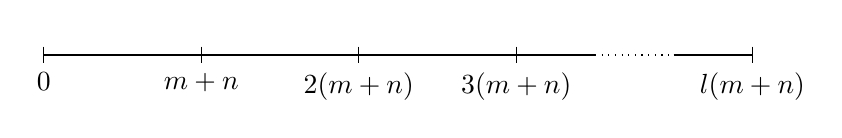
\begin{tikzpicture}

    \draw (0,0) -- (7,0);
	\draw[dotted] (7,0) -- (8,0);
	\draw (8, 0) -- (9, 0);
 
    \foreach \x in {0,2,4,6,9}
      \draw (\x cm,3pt) -- (\x cm,-3pt);

    \draw (0,0) node[below=3pt] {$ 0 $} node[above=3pt] {$   $};
    \draw (2,0) node[below=3pt] {$m+n$} node[above=3pt] {$  $};
    \draw (4,0) node[below=3pt] {$2(m+n)$} node[above=3pt] {$  $};
    \draw (6,0) node[below=3pt] {$3(m+n)$} node[above=3pt] {$ $};
	\draw (9,0) node[below=3pt] {$l(m+n)$} node[above=3pt] {$ $};
\end{tikzpicture}
\end{center}
Vsako zaporedje $\{X_l\}_{l \in \mathbb{N}}$ v $\widetilde{T}$ je zaporedje Bernoullijevih spremenljivk, saj pri upanju računamo verjetnost, da se v $m+n$ ponovitvah dogodek zgodi natanko $m+n$-krat. Torej $X_l$\textasciitilde $Ber(p^{m+n})$, medtem ko je zaporedje 
$\{X_l\}_{l \in \mathbb{N}}$ porazdeljeno geometrijsko, torej $G_l$\textasciitilde $Geom(p^{m+n})$, saj čakamo, da se dogodek, ko zaporedje vsebuje same enice, zgodi natanko enkrat. Sledi:

$$E[G_l]=\frac{1}{p^{(m+n)}} \Longrightarrow E[\widetilde{T}] = \frac{m+n}{p^{(m+n)}} < \infty$$
\end{frame}

\end{document}